\documentclass[10pt,landscape,a4paper]{article}
\usepackage{multicol}
\usepackage[landscape]{geometry}
\usepackage{amsmath,amsthm,amsfonts,amssymb, graphicx, physics}
\newcommand{\subs}[1]{\ensuremath{_{\text{#1}}}}
\newcommand{\rms}{\subs{rms}}
\newcommand{\nrms}[1]{\subs{#1,rms}}
\newcommand{\half}{\frac{1}{2}}
\newcommand{\inlineimage}[1]{\includegraphics[width=0.25\textwidth]{#1}\\}
\newcommand{\inlineimagesize}[2]{\includegraphics[width=#2\textwidth]{#1}\\}
\newcommand{\tise}{\ensuremath{-\frac{\hbar^2}{2m}\frac{1}{\psi}\frac{d^2\psi}{d\textbf{r}^2} + V = E}}
\newcommand{\minititle}[1]{\textbf{#1:}\\}
\renewcommand{\^}[1]{\ensuremath{\hat{#1}}}
\newcommand{\h}{\hbar}


% This sets page margins to 1cm
\geometry{top=1cm,left=1cm,right=1cm,bottom=1cm}

% Turn off header and footer
\pagestyle{empty}


% Don't print section numbers
\setcounter{secnumdepth}{0}

\setlength{\parindent}{0pt}
\setlength{\parskip}{0pt plus 0.5ex}
\begin{document}
	\begin{multicols}{4}
	\textbf{Cavity Radiation and the Ultraviolet Catastrophy}\\
	Reyleigh-Jeans: $ \rho_T(\nu) = \frac{8\pi\nu k_BT}{c^3}d\nu $\\
	Stefans Law: $ R_T = \sigma T^4 $, $ \sigma=\frac{2\pi^5k^4}{15c^2h^3} $, Wien's Displacement: $ \nu\subs{max}\propto~T $\\
	RJ is good fit at low frequencies, but assumption of equipartition is wrong, total energy is constant with atoms taking discrete energies in a Boltzmann distribution. $ \varepsilon ~ = ~ kT ~ \text{and}~P(\varepsilon) = \frac{e^{\frac{\varepsilon} {k_BT}}}{k_BT} $\\
	$ \Delta\varepsilon = h\nu $ so $ \bar{\varepsilon} = \frac{h\nu}{e^{\frac{h\nu}{k_BT}}-1} $\\
	\textbf{\textit{Plank's Radiation Law:}} \\
	$ \rho_T(\nu) = \frac{8\pi\nu^3}{c^3}\frac{h\nu}{e^{\frac{h\nu}{k_BT}}-1} $\\
	Photon energy: $ E = h\nu $, $ \hbar=\frac{h}{2\pi} $ Fine Structure constant: $ \alpha = \frac{e^2}{4\pi\epsilon_0\hbar c} $, Compton wavelength $ \lambda_C = \frac{h}{m_ec} $\\
	Newtonian assumes time is the same in all frames for all observers, special relativity assumes the speed of light is the same for all observers and frames.
	$ \gamma = \frac{1}{\sqrt{1-\beta}} $ and $ \beta=\frac{V}{c} $\\
	Invariant interval: $ \Delta s = c^2\Delta t^2 - \Delta x^2 $ $ >0 \implies $ time like, $ <0\implies $ space like, $ =0 \implies $ light like.\\
	Four vector: $ (c\Delta t,\Delta x,\Delta y,\Delta z)=( c\Delta t,\Delta \textbf{r}) $\\
	Inner Product: $ A\vdot B = A_0B_0 - \textbf{A}\vdot \textbf{B} \implies (\Delta s)^2 = c^2\Delta t^2 - \Delta x^2 $, the inner product of the space-time four vector is the invariant interval.\\
	Momentum, $ \textbf{p} = (\gamma mc, \gamma m\textbf{u}) $ and $ p = (\left(\frac{E}{c}\right),\textbf{p}) $ where $ E = \gamma mc^2 = mc^2 + KE $	
	\textbf{de Broglie:} $ E = h\nu $ so, $ p = \frac{h}{\lambda} $, \textbf{Uncertainty:} $ \Delta p \Delta x \geq \frac{\hbar}{2} $, $ \Delta E \Delta t \geq \frac{\hbar}{2} $ Phase velocity: $ \omega = \frac{dx_n}{dt}=\frac{\nu}{\kappa} $ Group velocity: $ g = \frac{d\nu}{d\kappa} $ \\
	\textbf{Heisenberg's Microscope:} To consider qualitatively the uncertainty principle, we will look at how we measure things, and how the measurement affects atomic particles.\\
	\inlineimage{hmicro.png}
	The light we observe has interacted off the incident proton, and has some uncertainty in x and movement (momentum).\\ 
	Diffraction limit: $ \Delta x = \frac{\lambda}{\sin(\epsilon/2)} $ (this is our uncertainty in x)\\
	There is also the uncertainty in momentum: $ \Delta p_x=\frac{h}{\lambda}[2\sin(\epsilon/2)] $, so the uncertainty product is constant: $ \Delta p_x \Delta x = 2h $\\
	\textbf{Philosophy of Quantum Physics:}\\
	\begin{itemize}
		\item Quantum is probabilistic in nature.
		\item There is no objective reality, making a measurement is the same thing as an interaction between two unobserved particles. These interactions collapse the superimposed wave forms, to the single outcome.
		\item Because of this, there is an uncertainty introduced. 
	\end{itemize}
	
	\textbf{Schrodinger's Equation}\\
	$ i\hbar \frac{\partial}{\partial t}\Psi(\textbf{r},t) = \hat{H}\Psi(\textbf{r},t) $\\
	This is just application of the Hamiltonian (energy) operator to the wave function of the particle. \\ 
	$ \bar{H} = \frac{\textbf{p}^2}{2m}+V = \frac{\hbar^2}{2m}(\frac{\partial}{\partial \textbf{r}})^2 + V $\\
	Splits into $ R(\textbf{r}) $ and $ T(t) $, and the time solution: $ T(t) = \frac{i\hbar}{E} e^{-iEt/\hbar} $\\
	\tise\\
	This is linear, meaning importantly that superposition of solutions and separation of variables are possible.\\
	\textbf{Normalisation} $ \int P d\tau = 1 $\\ $ \implies \int \Psi^*\Psi d\tau = 1 $ \\
	\textbf{Infinite Square Well:}\\
	\inlineimagesize{infsquarewell.png}{0.15}\\
	Boundary conditions, 1. Must be continuous and single valued everywhere.$ \int \Psi d\tau = 1 $ 3. $ \nabla\Psi $ continuous where V is continuous.\\
	Try a sinusoidal solution: $ \Psi(x) = A\cos kx + B\cos kx $, where $ k = \left(\frac{2mE}{\hbar}\right) $ but where $ V(x)=\infty $ the particle cannot exist, is $ \Psi(\pm a) = A\cos ka + B\sin ka = A\cos ka + B\sin (-ka) = 0 $ so we have solutions for $ A=0 $ and $ B=0 $ consisting of only odd, or only even solutions in $ n $. These solutions give the general case:
	\[ \sum_{n=1,3,5\ldots}^{\infty} A_n\cos(\frac{n\pi}{2a}x)+ \sum_{n=2,4,6\ldots}^{\infty} B_n\cos(\frac{n\pi}{2a}x) \] 
	Which scales by factor: $ A_n = B_n = a^{-1/2} $ and has associated with energy eigenvalues, $ E_n = \frac{\hbar^2\pi^2n^2}{8ma^2} $.\\
	\textbf{Finite square well,}, same solution for inside well, but the outside is the decay equation: $ \Psi(x) = Ce^{\pm\kappa x} $, which results in two sets of equations, the one relating to continuous case and the continuous gradient case.  \\
	So the solutions become: $ k\tan ka = \kappa = -k\cot ka $ where $ k=\sqrt{\frac{2mE}{\hbar^2}} $ and $ \kappa = \sqrt{\frac{2m}{\hbar^2}(V_0-E)} $, solved graphic/numerically.\\
	\textbf{Wave function sketching} rules come from this solution, $ k $ is proportional to the well depth and is related to energy, so shallow well high amplitude, low frequency. The height of the sides determines decay rate $ \kappa $. The number of nodes is $ n-1 $, parity of this is parity of the function.
	\textbf{Barrier tunnelling}, is the ability for particles to pass through an area of potential of higher energy than they possess. Related to the decay in a finite square well. A barrier of appreciable width $ b $ has tunneling probablility,	$ \frac{|F|^2}{|A|^2} = \frac{16k^2\kappa^2}{k^2+\kappa^2}e^{-2\kappa b} = \frac{16E(V_0-E )}{V_0^2}e^{-2\kappa b} $ which is a rate, $ \Gamma = \frac{n}{m}\hbar k \frac{|F|^2}{|A|^2}  $.\\
	\textbf{Example:} for $ \beta $ and $ \alpha $ decay, there is $ P_\text{trans} = \exp\left[\int_{r_\text{nuc}}^{r_\text{end}\frac{-2m}{\hbar^2}(V(r)-E)}\right] $\\
	\inlineimage{barriertunnelex.png}
	\textbf{Operators:}
	$ \hat{A}\Psi = a\Psi $\\
	Commutator: $ [\hat{A},\hat{B}] = \hat{A}\hat{B}-\hat{B}\hat{A} $
	Momentum: $ \hat{p}_z = -i\hbar\frac{\partial}{\partial z} $, Energy: $ \hat{T}_z= -\frac{\hbar^2}{2m}\frac{\partial^2}{\partial z^2} $ Angular Momentum: $ \hat{L}_z = -i\hbar\left(x\frac{\partial}{\partial y}-y\frac{\partial}{\partial x}\right) $, Potential Energy: $ \hat{V}_z = V(z) $, Hamiltonian: $ \hat{H}_z = \hat{T}_z+\hat{V}_z $\\
	Complex Conjugates: $ \hat{Q}^*f^* = \left(\hat{Q}f\right)^* $ Hermitian operators: $ \int f\hat{Q}gd\tau = \int g\hat{Q}^*fd\tau $ with real eigenvalues, and orthonormal eigenvectors, $ 
	\int\phi^*_n\phi_md\tau = \delta_{nm} $ scaled so that: $ \int|\phi_n|^2d\tau = 1 $\\
	Coefficients: $ a_n = \int\phi^*_n\psi d\tau $\\
	\inlineimage{postulates.png}
	\textbf{Uncertainty:}\\
	Observations are compatible if they are governed by the same set of eigenfunctions.\\
	$ \hat{Q}^\prime = (\hat{Q} - \expval*{\hat{Q}}) $ so the deviation compared to the expected result is defined. This means that the standard deviation is the expectation value of this.
	$ \Delta q^2 = \int \psi^*\hat{Q}^\prime\hat{Q}^\prime\psi d\tau $\\
	so the deviation product: $ \Delta q\Delta r \ge \frac{1}{2}\left|\int\psi^*\left[\hat{Q},\hat{R}\right]\psi d \tau\right|^2 $\\
	\minititle{Degeneracy}
	If $ \hat{Q}\phi_n = p_n\phi_n $ then $ q_n\neq q_m $ for all $ n\neq m $. Is the requirement that must be modified.\\
	If $ \hat{Q} $ acting on $ \phi_1 $ and $ \phi_2 $ are degenerate in the eigenvalue $ q $ and commute with $ \hat{R} $. Then there is some linear combination of these eigenvectors that equate to the eigenvector of $ \hat{R} $, $ \phi^\prime_n $. ie: $ \hat{R}\phi^\prime_n = r_n\phi^\prime_n = r_n\left(C_1\phi_1+C_2\phi_2\right) $
	
	\minititle{Ladder Operators}
	$ (\^P^2+\^X^2 ) \overset{?}{=} (\^P + i\^X)(\^P-i\^X) $ so let $ \^A = (\^P-i\^X) $ and $ \^A^\dagger = (\^P + i\^X) $ so $ \^H = \half(\^A^\dagger\^A+1) = \half(\^A\^A^\dagger-1) $
	So the commutators, $ \left[\^A,\^H\right] = \^A\half(\^A^\dagger\^A + 1) - \half(\^A\^A^\dagger - 1)\^A = \^A $ So when the commutator operates on the wave function, $ \^H\^A^\dagger\psi = (E_n-1)\psi $ So this is the lowering operator and $ \^H\^A\psi_0 = \half\psi_0 $\\
	\minititle{Angular Momentum}
	$ \left[\^L_x,\^L_y\right] = \^Y\^P(\^P_z\^Z-\^Z\^P_z) + \^X\^P_y(\^Z\^P_z - \^P_z\^Z) = i\hbar\^L_z $, or in general: $ \left[\^L_i,\^L_j\right] = i\hbar\varepsilon_{ijk}\^L_k $ where	levi cevita:\\
	$ \epsilon_{xyz} = 1 \\
	\epsilon_{xxz} = 0 \\	
	\epsilon_{yxz} = -1 $\\
	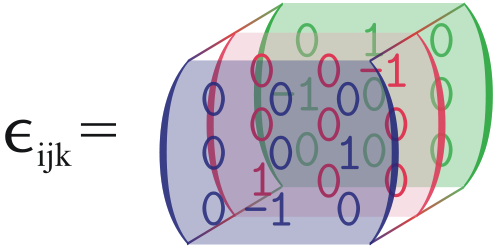
\includegraphics[width=0.2\textwidth]{levicevita.png}\\
	$ \^L_i $ and $ \^L_j $, $ \^P_j $ or $ \^X_j $ are incompatible, but $ \^L^2 $ and $ \^L_i $ or $ \^H $ are compatible.\\ 
	\minititle{Spherical Coordinates}
	$ \frac{\partial}{\partial x} = \sin\theta\cos\phi\frac{\partial}{\partial r} + \frac{\cos\theta\cos\phi}{r} \pdv{\theta} - \frac{\sin\phi}{r\sin\theta}\pdv{\phi} $ \\
	$ \pdv{y} = \sin\theta\sin\phi\pdv{r} + \frac{\cos\theta\sin\phi}{r}\pdv{\theta} + \frac{\cos\phi}{r\sin\theta}\pdv{\phi} $\\
	$ \pdv{z} = \cos\theta\pdv{r} - \frac{\sin\theta}{r}\pdv{\phi} $\\
	So the grad operator becomes: $ \grad = r_0\pdv{r}+\frac{1}{r}\theta_0\pdv{\theta} + \frac{1}{r\sin\theta}\phi_0\pdv{\phi} $\\
	$ \^L = -i\hbar \vb*{r}\cross\grad = -i\hbar\left(\phi_0\pdv{\theta} - \frac{1}{\sin\theta}\theta_0\pdv{\phi}\right) $\\
	$ \^L_z = -i\hbar\pdv{\phi} $ \\
	$ \^L^2 = -\hbar^2\left[\frac{1}{\sin\theta}\pdv{\theta}(\sin\theta\pdv{\theta}) + \frac{1}{\sin^2\theta}\pdv[2]{\phi} \right] $\\
	\minititle{Polar Schrodinger}
	\[ -\frac{\hbar^2}{2\mu}\left[\frac{1}{r^2}\pdv{r}\left(r^2\pdv{\psi}{r}\right) + \frac{1}{r^2\sin\theta}\pdv{\theta}\left(\sin\theta\pdv{\psi}{\theta}\right) + \frac{1}{r^2\sin^2\theta}\pdv[2]{\psi}{\phi} \right] + V(r)\psi = E\psi \]
	Which has solutions: \\
	$ Y_{lm}(\theta,\phi) = (-1)^m\left[\frac{(2l+1)(l-|m|)!}{4\phi(l+|m|)!}\right]^\half e^{im\phi}$\\ 
	Which normalised become:\\
	\inlineimagesize{sphericalsoln.PNG}{0.15}\\
	$ l $ and $ m $ are important because they show the eigenvalues of $ \^L^2 $ and $ \^L_z $ respectively. \\
	\minititle{Angular Momentum as Vectors}
	\inlineimagesize{angularmomentvector.png}{0.15}
	\textbf{The Bohr Magneton} $ \mu_B \equiv \frac{\mu\hbar}{2m_e} $ yielding a $ \Delta E = \mu B m\h $\\
	\minititle{Ladder operators and Angular Moment}
	$ \^L_+ = \^L_x+i\^L_y $ and $ \^L_- = \^L_x - i\^L_y $ and their commutator, $ \left[\^L_+,	\^L_-\right] = 2\h\^L_z $, and they don't commute with $ \^L_z $.\\
	Using this operator: $ \^L_z\^L_+\phi = (m+1)\h\phi $ but the raising and lowering operators commute with $ \^L^2 $ so the eigenfunction/total angular momentum is unchanged.\\
	\minititle{Semi-classical $ \mu_B $}
	$ \mu_l = \sqrt{l(l+1)}g_l\mu_b $ and $ \mu_{l_z} = -g_l\mu_bm_l $\\ \\ \\ \\
	\textbf{Larmor precession:} $ \omega = \frac{g_l\mu_b}{\h}B $
	\textbf{Particle Spin:} $ S = \sqrt{s(s+1)}\h = \frac{\sqrt{3}\h}{2} $, so $ S_z = m_s\h $, where $ m_s = \pm \half $, so the moments: $ \mu_s = -\frac{e}{m}S $ and $ \mu_{S_z} = -2m_s\mu_b $\\
	These new operators commute with the old angular momentum operators. Hence they introduce new degeneracies in to the equations.\\
	\minititle{Matrix Eigenvalue equation}
	$ \begin{pmatrix}
	Q_{11} & Q_{12} & Q_{13}\\
	Q_{21} & Q_{22} & Q_{23}\\
	Q_{31} & Q_{32} & Q_{33}\\
	\end{pmatrix} \begin{pmatrix}
	a_1\\a_2\\a_3
	\end{pmatrix} = q\begin{pmatrix}
	a_1\\a_2\\a_3
	\end{pmatrix} $\\
	The Hermitian requirement means, $ Q_{mn} = Q^*_{nm} $ and $ [Q] = [Q^\dagger] $.\\
	$ \mdet{Q_{11}-q & Q_{12} & Q_{13}\\Q_{21} & Q_{22}-q & Q_{23}\\Q_{31} & Q_{32} & Q_{33}-q} = 0 $\\
	Are the solutions.\\
	\minititle{Pauli Spin Matrices}
	$ \sigma_x = \mqty[0 & 1 \\ 1 & 0]~~\sigma_y = \mqty[0 & -i \\ i & 0]~~\sigma_z=\mqty[1 & 0 \\ 0 & -1] $\\
	So the spin operator becomes, $ \^S_x = \half\h\sigma_x $, etc.
	and the angular momentum operators become,	$ \^L^2 = 2\h^2\sbmqty{1&0&0\\0&1&0\\0&0&1} $ and $ \^L_z = \h\sbmqty{1&0&0\\0&0&0\\0&0&-1} $, the raising operators, $ \^L_+ = \sbmqty{0&\sqrt{2}&0\\0&0&\sqrt{2}\\0&0&0} $ and $ \^L_- = \h\sbmqty{0&0&0\\0&0&\sqrt{2}\\0&\sqrt{2}&0} $
	\minititle{Dirac Notation}
	\inlineimage{intergralnotation.png}
	\inlineimage{diracnotation.png}
	\minititle{Spin Orbit Interaction}
	By considering the Biot-Savart Law, gives a potential difference due to the internal \textbf{B} field.
	$ U_{LS} = -\mu_s\vdot B = \frac{1}{2m^2c^2r}\dv{V(r)}{r}S\vdot L $\\
	The interaction means they are not independent, resulting a new quantum number $ \^J = \sqrt{j(j+1)}\h $, and $ \^J_z = m_j\h $, which in the $ z $ direction is, $ \^J_z = m_l+m_s $.\\
	This gives a degeneracy the energies that sum to the total $ J $,
	\[ \ket{j,m_j} = \sum_{m_l}\sum_{m_s}C_{j,m_j,m_l,m_s}\ket{m_l}\ket{m_s} \]
	The largest value of this is $ \^J_z = \^L_z + \^S_z $, ie $ j = l\pm\half $. and the separations,
	$ \expval{E} = \frac{\h^2}{4m^2c^2r}\left(\frac{1}{r}\dv{V(r)}{r}\right)^* $\\
	\minititle{Zeeman Effect}
	The spin-orbit Hamiltonian, $ \^H' = \frac{1}{4m_e^2c^2r}\pdv{V}{r}(\^J^2-\^L^2-\^S^2) +\frac{\mu_b}{\h}B_0(\^L_z+2\^S_z) $ in no external field, this becomes simply, $ (\^J^2-\^L^2-\^S^2) = [j(j+1)-l(l+1)-s(s+1)]\h^2 $. When the magnetic field is much larger, the energy shifts become, $ \delta E = \mu_bB(m_l+2m_s) $\\
	
	\minititle{Perturbation theory}
	To the first order: $ \^H = (\^H_0+\lambda\^H) \implies (\^H_0 + \lambda\^H)\psi = E\psi $\\
	The eigenfunction's are then $ \psi_n = \phi_{0n} + \lambda\phi_{1n} + \lambda^2\phi_{2n} + \ldots $ and the energy values: $ E_n = E_{0n} + \lambda E_{1n} + \lambda^2 E_{2n} + \ldots $\\
	So the first order perturbation: $ \^H^\prime\phi_{0n} + \^H_0\phi_{1n} = E_{0n}\phi_{1n}+E_{1n}\phi_{0n} $ so the n'th order correction is the sum of the unperturbed system and the n'th order perturbation, then the energy is $ E\uparrow $ and $ \phi\downarrow $.\\
	$ \lambda E^{(1)}_n = \expval{\lambda H^\prime} = \bra{\phi_n}\lambda\^H^\prime\ket{\phi_n} $\\
	Second order correction: $ E^{(2)}_n = \sum_{k\ne n} \frac{|\bra{\phi_k}\lambda\^H^\prime\ket{\phi_n}|^2}{E_{0n}-E_{0k}} $ This second order shift will result in a spreading out of these levels.\\
	$ \psi_n = \phi_n+\sum_{k\ne n}\frac{\bra{\phi_k}\^H^\prime\ket{\psi_n}}{E_{0n}-E_{0k}}\phi_k $\\
	Doesn't work for degeneracies. $ E-E = 0 $\\
	\minititle{Sudden Approximation}
	$ \^H = \left\{ \mqty{\^H_1~~,t<0 \\ \^H_2~~,t\ge 0} \right. $\\
	\minititle{Fermi's golden rule} for transition rates between states m and n, $ \Gamma_{mn} = \frac{2\pi}{\h}\delta(E_n-E_m)|\^H^{\prime\prime}|^2 $ the delta function is cancelled in the integration of over a range of energies, $ \int\Gamma_{mn}\rho(E_n)dE_n = \frac{2\pi}{\h}\rho(E_m)|\^H^{\prime\prime}|^2 $\\
	\minititle{Ehrenfest Theorem}
	$ \pdv{\expval{\^Q}}{t} = \frac{i}{\h}\expval{\comm\big{\^H}{\^Q}}+\expval{\pdv{\^Q}{t}} $
	Ehrenfest states that the rate of change of the expectation value of a physical quantity has two factors, the commutator with the Hamiltonian, and the expectation value of the time derivative.\\
	EG. $ \pdv{\expval*{\^X}}{t} = \frac{\expval*{\^P}}{m} $\\
	\minititle{Cross Section}
	Differential cross section is the fraction of incident particles scattered per unit solid angle, $ \dv{\sigma}{\Omega} $\\
	Classically, for a hard sphere: $ \dv{\sigma(\theta)}{\Omega} = \frac{R^2}{4} $ and $ \sigma = \int\dv{\sigma(\theta)}{\Omega}d\Omega = \pi R^2  $\\
	In quantum, $ \Gamma = \frac{\h k}{mL} $ and the particle probability, $ \Gamma(x_2)-\Gamma(x_1) = \pdv{P}{t} = \dv{t}\left(\int_{x_1}^{x_2}\psi^*\psi dx\right) = \int_{x_1}^{x_2}\left(\psi^*\pagebreak\dv{\psi}{t}+\dv{\psi^*}{t}\psi\right)dt $\\
	So the flux is, $ \Gamma(x) = -\frac{i\h}{2m}\qty(\psi^*\pdv{\psi}{t}-\pdv{\psi^*}{t}\psi) $\\
	\minititle{Born Approximation}
	The scatterer is a perturbation to the incident wave is an elastic scattering example, with transition rate, $ W = \frac{2\pi}{\h^2}|V_{k_1,k_0}|^2 g(\omega) $, where $ V_{k_1 k_0} = \int\psi^*_f V(r)\psi_i d\tau $ and $ dg = \frac{mk\left[Volume\right]}{8\pi^3\h}d\Omega $ describes the density of states.\\
	\textbf{Differential cross section for a free particle and a radial perturbing potential,} $ \dv{\sigma}{\Omega} (\theta,\phi) = \left(\frac{m}{2\pi\h^2}\right)^2\left|\int V(r)e^{-iK\vdot r}d\tau \right|^2 $\\
	\minititle{Partial Wave}
	Now we care about the phase shifts induced by the scatterer and the angular momentum of the particle. $ dN = \frac{\h k}{mV}\abs{f(\theta)}^2d\Omega \implies \dv{\sigma}{\Omega} = \abs{f(\theta)}^2 $ so the total cross section: $ \sigma = 2\pi\int_0^\pi |f(\theta)|^2\sin\theta d\Omega $. Which for our radial electric potential is, $ \frac{4\pi}{k^2}\sum(2l+1)\sin^2\delta_l $ over all $ l $, however $ \delta_l $ is hard to get, except for when $ l=0 $.
	
	\end{multicols}
	\begin{multicols}{2}
		\minititle{Examples}
		\inlineimagesize{q1ai.png}{0.5}
		
		\minititle{q2a}
		\inlineimagesize{q2ai.png}{0.5}
		$ \therefore E = \frac{p^2}{2m} \implies p = \sqrt{2mE}\\
		\int p dq = nh \implies \int p dq + \int -p dq = 2\int \sqrt{2mE} dx\\
		2\sqrt{2mE}r_0 = nh \therefore E = \frac{h^2n^2}{8mr_0^2} $
		
		\minititle{q2b}
		$ X^*_2 \rightarrow X_2 + \gamma \\
		E^2 - c^2p^2 = m^2c^4 \\
		\gamma \implies m=0 \therefore E^2 = c^2p^2 $\\
		Sketch the vector sum.\\
		Show $ E_\gamma = \half\frac{(m_*^2-m^2)c^4}{m_*c^2}\\ $
		Conservation of energy: $ E_* = E_m + E_\gamma $\\
		Convervation of momentum: $ p_* = p_m+p_\gamma = 0 $\\
		So from mass shell and squaring above: $ m_*^2c^4-0^2c^2 =E_m^2+E_\gamma^2+2E_mE_\gamma-c^2(p_m^2+p_\gamma^2-2p_\gamma^2) $ \\
		Rearrange for $ 2E_mE_\gamma = m_*^2c^4 - (E_m^2-c^2p_m^2) - (E_\gamma^2-c^2p_\gamma^2) -2c^2p_\gamma^2 $ which are the 2 mass shells, $ \therefore = m_*^2c^4 $ and $ = m^2c^4 $\\
		$ \therefore 2E_mE_\gamma = m_*^2c^4 - m^2c^4-2p_\gamma $\\
		Sub $ E_m $ from conservation of energy. Solve for $ E_\gamma $\\
	\end{multicols}
\end{document}